% ==============================================================================
% PLANTILLA MAESTRA DE REPORTE ACADÉMICO - UANL
% Universidad Autónoma de Nuevo León
% ==============================================================================
% Uso rápido:
% 1) Duplica esta plantilla y renombra la copia según la actividad o evidencia:
%    ej. reporte-biologia-celular-PIA.tex, reporte-calculo-Actividad-1.tex.
% 2) Actualiza \documenttitle, \documentsubtitle, \documentsubject, \coursename,
%    \universityfaculty, datos del estudiante y del profesor.
% 3) Configura el logotipo de la facultad en \universitydepartmentimage:
%    - Para Facultad de Agronomía: departamentos/logo-agronomia
%    - Para FIME: departamentos/logo-fime
%    - Para UANL institucional general: departamentos/logo-uanl
% 4) Lee la planeación de Nexus/AulaTeX y NO pegues las instrucciones textuales
%    dentro del PDF. Úsalas como lista de verificación y redacta con criterio propio.
% 5) Elabora productos visuales preferentemente en LaTeX/TikZ o tablas booktabs
%    para garantizar nitidez y trazabilidad profesional.
% 6) Compilar con:
%    powershell -File .\aulaTEX\latexmk-build.ps1 .\UANL\reporte-uanl.tex
%
% Formato institucional:
% - Tipografía: Helvetica / sans-serif equivalente (\usepackage{helvet}).
% - Interlineado: 1.5 (\onehalfspacing integrado en el motor de plantilla).
% - Citas: autor-año natbib (\citep{clave}, \citet{clave}) en APA 7ma edición.
% - Bibliografía: vinculada a bibliografia-uanl.bib o archivo .bib de la materia.
% - Estructura mínima: Portada institucional UANL, Resumen/Abstract, Índice,
%   Introducción, Desarrollo analítico, Producto visual, Conclusión argumentada
%   con transferencia profesional y Referencias.
% ==============================================================================

\documentclass[
	spanish,
	letterpaper, oneside
]{article}

% ==============================================================================
% INFORMACIÓN DEL DOCUMENTO Y METADATOS ACADÉMICOS
% ==============================================================================
\def\documenttitle {Reporte Académico Institucional UANL}
\def\documentsubtitle {Plantilla Maestra de Evidencias y Productos Integradores (PIA)}
\def\documentsubject {Unidad de Aprendizaje Curricular}

\def\documentauthor {Carlos Mauricio Carvajal Coronado}
\def\coursename {Biología Celular}
\def\coursecode {REF\#261013755061}

\def\universityname {Universidad Autónoma de Nuevo León}
\def\universityfaculty {Facultad de Agronomía}
\def\universitydepartment {Programa Educativo de Ingeniero Agrónomo}
\def\universitydepartmentimage {departamentos/logo-agronomia}
\def\universitydepartmentimagecfg {height=1.57cm}
\def\universitylocation {General Escobedo, Nuevo León}

% ==============================================================================
% TABLA DE INTEGRANTES, PROFESORES Y FECHAS
% ==============================================================================
\def\authortable {
	\begin{tabular}{ll}
		\textbf{Estudiante:} & Carlos Mauricio Carvajal Coronado \\
		\textbf{Matrícula:}  & 1977875 \\
		\textbf{Profesor:}   & Dr. Miguel Ángel Dector Carrillo \\
		& \\
		\multicolumn{2}{l}{Fecha de elaboración: \today} \\
		\multicolumn{2}{l}{\universitylocation}
	\end{tabular}
}

% ==============================================================================
% IMPORTACIÓN DEL TEMPLATE BASE DE AULATEX
% ==============================================================================
\input{template_config}
\input{template}

% PAQUETES COMPLEMENTARIOS PARA MAQUETACIÓN PROFESIONAL
\usepackage{helvet}
\renewcommand{\familydefault}{\sfdefault}
\usepackage{booktabs}
\usepackage{array}
\usepackage{longtable}
\usepackage{tikz}
\usetikzlibrary{arrows.meta,calc,positioning,shapes.geometric,shadows.blur}

% CONFIGURACIÓN DE CITAS EN FORMATO AUTOR-AÑO (APA 7)
\setcitestyle{authoryear,open={(},close={)}}

% PALETA CROMÁTICA INSTITUCIONAL UANL
\definecolor{uanlBlue}{HTML}{00376C}
\definecolor{uanlGold}{HTML}{D4AF37}
\definecolor{uanlGreenAgro}{HTML}{1B5E20}
\definecolor{uanlPaper}{HTML}{F6F8F7}

% ==============================================================================
% INICIO DEL DOCUMENTO
% ==============================================================================
\begin{document}

% PORTADA INSTITUCIONAL
\templatePortrait

% CONFIGURACIÓN DE PÁGINA Y ENCABEZADOS FORMALES
\templatePagecfg

% RESUMEN / ABSTRACT
\begin{abstractd}
El presente reporte académico establece la estructura metodológica, analítica y documental normalizada para la entrega de evidencias de aprendizaje y Productos Integradores de Aprendizaje (PIA) en la Universidad Autónoma de Nuevo León (UANL). La propuesta articula el rigor científico, el marco formativo del Modelo Educativo institucional y los lineamientos de excelencia editorial de AulaTeX. A través de una delimitación precisa del objeto de estudio, análisis crítico con soporte empírico y bibliográfico, y transferencia directa a la práctica agronómica y profesional, se garantiza un estándar homogéneo de comunicación científica, trazabilidad analítica y solvencia técnica.
\end{abstractd}

% ÍNDICE DE CONTENIDOS
\templateIndex

% CONFIGURACIONES FINALES DE PÁGINA
\templateFinalcfg

% ==============================================================================
% DESARROLLO DEL CONTENIDO
% ==============================================================================

\section{Introducción y Justificación Académica}

El desarrollo de competencias en los programas académicos de la Universidad Autónoma de Nuevo León exige que las actividades de aprendizaje superen la recopilación descriptiva y se constituyan en ejercicios genuinos de interpretación científica, diagnóstico técnico y juicio profesional fundamentado \citep{uanlModeloEducativo2022}. De acuerdo con la visión estratégica universitaria orientada hacia la sociedad del conocimiento \citep{uanlVision2030}, el estudiante debe ser capaz de analizar problemáticas reales del entorno biológico, agropecuario, industrial o tecnológico, respaldando cada tesis de trabajo con literatura indexada y normativa vigente.

La presente plantilla institucional provee el andamiaje compositivo para estructurar reportes de laboratorio, estudios de caso, artículos de revisión bibliográfica y proyectos integradores. Su diseño balancea la identidad corporativa de la UANL (representada por sus colores emblemáticos azul y oro, y el verde agropecuario distintivo de la Facultad de Agronomía) con la legibilidad tipográfica y la precisión requerida en publicaciones técnicas.

\section{Marco Teórico y Fundamentación Conceptual}

Toda evidencia académica de nivel superior requiere fundamentar sus postulados en tratados de referencia y publicaciones de arbitraje riguroso. En el ámbito de las ciencias biológicas, agronómicas y de ingeniería, la integración de principios ultraestructurales, bioenergéticos y fisiológicos permite explicar fenómenos macroscópicos a partir de mecanismos celulares y moleculares discretos \citep{albertsMolecularBiology2022,nelsonLehningerBiochemistry2021}.

\subsection{Principios Fisiológicos y Respuestas Adaptativas}
Los sistemas vivos responden a gradientes biofísicos y señales ambientales a través de cascadas moleculares altamente integradas. Por ejemplo, en los tejidos vegetales, la modulación del potencial hídrico foliar y la regulación del intercambio gaseoso constituyen mecanismos primordiales para optimizar la eficiencia del uso del agua frente a escenarios de estrés por sequía o salinidad \citep{taizPlantPhysiology2015,karpBiologiaCelular2019}. 

\subsection{Trazabilidad Metodológica}
Conforme a las pautas metodológicas de la investigación aplicada \citep{hernandezSampieriMetodologia2018}, el análisis formal debe especificar:
\begin{enumerate}
	\item \textbf{Criterio de observación:} Identificación de variables independientes, dependientes y condiciones de control ambiental o experimental.
	\item \textbf{Instrumentación y técnica:} Procedimientos instrumentales, métodos de simulación numérica o protocolos analíticos aplicados.
	\item \textbf{Criterio de validación:} Evaluación de coherencia teórica, límites termodinámicos y significancia en el contexto agronómico o ingenieril.
\end{enumerate}

\section{Análisis de Resultados y Evidencia Visual}

Para garantizar nitidez y reproducibilidad vectorial, los productos visuales y cuadros comparativos deben elaborarse en entornos nativos de LaTeX (como `booktabs` o `TikZ`), evitando capturas rasterizadas de baja resolución.

\subsection{Matriz Comparativa de Desempeño y Criterios Operativos}
En el Cuadro~\ref{tab:criterios_uanl} se sintetizan los componentes estructurales mínimos requeridos en las entregas académicas institucionales de la UANL.

\begin{table}[htbp]
	\centering
	\small
	\caption{Matriz de criterios estructurales y niveles de dominio de AulaTeX en UANL.}
	\label{tab:criterios_uanl}
	\begin{tabular}{p{0.25\linewidth} p{0.35\linewidth} p{0.32\linewidth}}
		\toprule
		\textbf{Componente} & \textbf{Criterio de Realización} & \textbf{Impacto Formativo} \\
		\midrule
		\textbf{Rigor conceptual} & Definición precisa de principios biológicos o ingenieriles sin vaguedades. & Evita la confusión terminológica y consolida vocabulario técnico. \\
		\addlinespace
		\textbf{Soporte bibliográfico} & Inclusión obligatoria de citas autor-año en APA 7 vinculadas a `bibliografia-uanl.bib`. & Asegura trazabilidad y combate el plagio académico. \\
		\addlinespace
		\textbf{Evidencia visual} & Construcción de esquemas y cuadros en `TikZ` o `booktabs`. & Facilita la interpretación analítica y la defensa oral. \\
		\addlinespace
		\textbf{Transferencia profesional} & Vinculación explícita con el rendimiento de cultivos, sostenibilidad o industria. & Demuestra pertinencia social del egresado UANL. \\
		\bottomrule
	\end{tabular}
\end{table}

\subsection{Esquematización Vectorial con TikZ}
A continuación, la Figura~\ref{fig:flujo_aulatex} ilustra la arquitectura de trabajo descendente de AulaTeX aplicada a las unidades de aprendizaje de la UANL.

\begin{figure}[htbp]
	\centering
	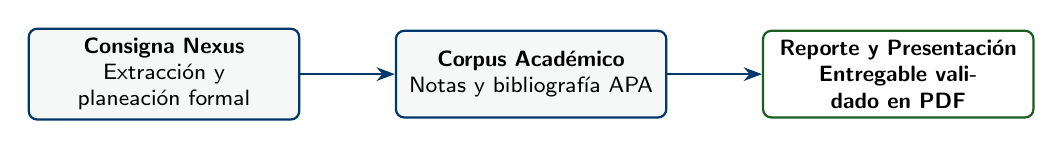
\begin{tikzpicture}[
		node distance=1.6cm,
		block/.style={
			rectangle,
			draw=uanlBlue,
			fill=uanlPaper,
			thick,
			rounded corners=3pt,
			text width=3.2cm,
			align=center,
			minimum height=1.1cm,
			font=\footnotesize\sffamily
		},
		accentblock/.style={
			rectangle,
			draw=uanlGreenAgro,
			fill=white,
			thick,
			rounded corners=3pt,
			text width=3.2cm,
			align=center,
			minimum height=1.1cm,
			font=\footnotesize\sffamily\bfseries
		},
		line/.style={
			draw=uanlBlue,
			-Stealth,
			thick
		}
	]
		\node[block] (consigna) {\textbf{Consigna Nexus}\\ Extracción y planeación formal};
		\node[block, right=1.2cm of consigna] (corpus) {\textbf{Corpus Académico}\\ Notas y bibliografía APA};
		\node[accentblock, right=1.2cm of corpus] (producto) {Reporte y Presentación\\ Entregable validado en PDF};

		\path[line] (consigna) -- (corpus);
		\path[line] (corpus) -- (producto);
	\end{tikzpicture}
	\caption{Flujo metodológico de desarrollo de evidencias bajo contratos de AulaTeX.}
	\label{fig:flujo_aulatex}
\end{figure}

\section{Conclusiones y Transferencia Profesional}

La adopción de una plantilla institucional normalizada en la UANL cumple una doble función formativa: por una parte, eleva el estándar editorial y estético de las entregas de los estudiantes hacia niveles homologables con publicaciones indexadas; por otra, promueve un hábito de pensamiento estructurado donde cada afirmación está respaldada por evidencia empírica y literatura científica verificable.

En el contexto específico de la agronomía y las ingenierías afines, la habilidad para redactar reportes técnicos rigurosos, procesar información bibliográfica con normas internacionales (APA 7ma edición) y sintetizar conclusiones orientadas a la toma de decisiones representa un diferenciador profesional determinante para el egresado de la Universidad Autónoma de Nuevo León frente a los retos de la productividad agroalimentaria sostenible y el cambio climático.

% ==============================================================================
% REFERENCIAS BIBLIOGRÁFICAS
% ==============================================================================
\clearpage
\bibliography{bibliografia-uanl}

\end{document}
